\begin{figure*}[t]
    \centering
    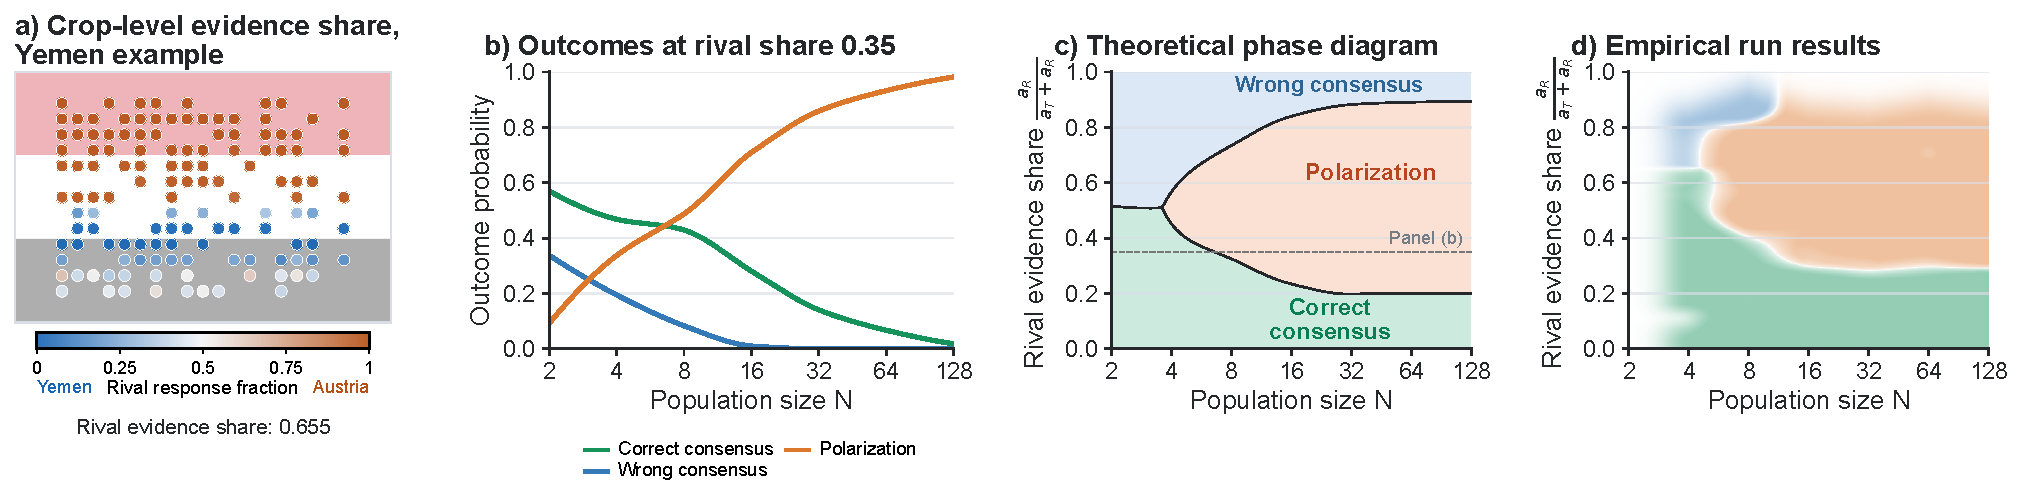
\includegraphics[width=\textwidth]{../paper/figures/final/fig8.pdf}
    \caption{\textbf{Private evidence and collective outcomes across population sizes.}
    (a) Rival response fractions from 50 binary probes per crop in a Yemen run
    ($N=128$, seed 0020): blue is 0 (Yemen), orange is 1 (Austria).
    Pooling the crop responses gives rival evidence share $4192/6400=0.655$.
    (b) Exact endpoint probabilities for the binary copying model
    at rival evidence share $0.35$.
    In the binary theory, consensus requires at least 85\% agreement;
    all remaining splits count as polarization.
    (c) Theoretical phase diagram versus population size and rival evidence share
    $a_R/(a_T+a_R)$; regions show the most probable outcome and the dashed line
    marks (b). Curves interpolate calculations at $N=2,4,8,16,32,64,128$.
    Boundaries mark probability crossings, not thermodynamic transitions.
    (d) Empirical run results from 217 runs, using each run's rival evidence share. Regions show the locally most frequent outcome,
    estimated independently of the theory with Gaussian bandwidth $0.05$ in share.
    Empirical classifications retain the 25\% threshold for each of at least two
    countries to count as polarization, with remaining non-consensus outcomes
    classified as fragmentation.
    Panels b--c use $a_T+a_R=0.45$ and $h_0=+0.3$.}
    \label{fig:theory-four-panel}
\end{figure*}
